% Options for packages loaded elsewhere
\PassOptionsToPackage{unicode}{hyperref}
\PassOptionsToPackage{hyphens}{url}
%
\documentclass[
]{article}
\usepackage{amsmath,amssymb}
\usepackage{lmodern}
\usepackage{iftex}
\ifPDFTeX
  \usepackage[T1]{fontenc}
  \usepackage[utf8]{inputenc}
  \usepackage{textcomp} % provide euro and other symbols
\else % if luatex or xetex
  \usepackage{unicode-math}
  \defaultfontfeatures{Scale=MatchLowercase}
  \defaultfontfeatures[\rmfamily]{Ligatures=TeX,Scale=1}
\fi
% Use upquote if available, for straight quotes in verbatim environments
\IfFileExists{upquote.sty}{\usepackage{upquote}}{}
\IfFileExists{microtype.sty}{% use microtype if available
  \usepackage[]{microtype}
  \UseMicrotypeSet[protrusion]{basicmath} % disable protrusion for tt fonts
}{}
\makeatletter
\@ifundefined{KOMAClassName}{% if non-KOMA class
  \IfFileExists{parskip.sty}{%
    \usepackage{parskip}
  }{% else
    \setlength{\parindent}{0pt}
    \setlength{\parskip}{6pt plus 2pt minus 1pt}}
}{% if KOMA class
  \KOMAoptions{parskip=half}}
\makeatother
\usepackage{xcolor}
\usepackage[margin=1in]{geometry}
\usepackage{graphicx}
\makeatletter
\def\maxwidth{\ifdim\Gin@nat@width>\linewidth\linewidth\else\Gin@nat@width\fi}
\def\maxheight{\ifdim\Gin@nat@height>\textheight\textheight\else\Gin@nat@height\fi}
\makeatother
% Scale images if necessary, so that they will not overflow the page
% margins by default, and it is still possible to overwrite the defaults
% using explicit options in \includegraphics[width, height, ...]{}
\setkeys{Gin}{width=\maxwidth,height=\maxheight,keepaspectratio}
% Set default figure placement to htbp
\makeatletter
\def\fps@figure{htbp}
\makeatother
\setlength{\emergencystretch}{3em} % prevent overfull lines
\providecommand{\tightlist}{%
  \setlength{\itemsep}{0pt}\setlength{\parskip}{0pt}}
\setcounter{secnumdepth}{-\maxdimen} % remove section numbering
\usepackage{cancel}
\ifLuaTeX
  \usepackage{selnolig}  % disable illegal ligatures
\fi
\IfFileExists{bookmark.sty}{\usepackage{bookmark}}{\usepackage{hyperref}}
\IfFileExists{xurl.sty}{\usepackage{xurl}}{} % add URL line breaks if available
\urlstyle{same} % disable monospaced font for URLs
\hypersetup{
  pdftitle={Caso Gamma revisto},
  pdfauthor={Silvaneo Viera dos Santos Junior},
  hidelinks,
  pdfcreator={LaTeX via pandoc}}

\title{Caso Gamma revisto}
\usepackage{etoolbox}
\makeatletter
\providecommand{\subtitle}[1]{% add subtitle to \maketitle
  \apptocmd{\@title}{\par {\large #1 \par}}{}{}
}
\makeatother
\subtitle{Relatório}
\author{Silvaneo Viera dos Santos Junior}
\date{2022-11-23}

\begin{document}
\maketitle

\hypertarget{priori-alternativa-para-o-modelo-gamma}{%
\subsection{Priori alternativa para o modelo
Gamma}\label{priori-alternativa-para-o-modelo-gamma}}

Neste relatório apresentaremos um \emph{follow-up} das análises feitas
sobre o GDLM k-paramétrico para o caso Gamma com parâmetro de forma e
média desconhecidos. Durante a última reunião, observamos que a
compatibilização de prioris estava gerando uma aproximação ruim e foi
levantada a suspeita de que a isso estaria ocorrendo por causa de
restrições feitas ao espaço paramétrico afim de obter soluções para o
sistema de compatibilização de prioris.

Após a reunião, refletindo mais sobre o assunto, encontrei percebi que o
problema estava na escolha da priori, especificamente, a escolha do
modelo observacional
\(X|\alpha,\beta \sim \mathcal{G}\left(\alpha,\beta\right)\) me levou a
escolher uma parametrização ruim para a priori. Ao trabalhar com o
modelo observacional
\(X|\phi,\mu \sim \mathcal{G}\left(\phi,\frac{\phi}{\mu}\right)\) a
priori ``natural'', é bem mais tratável. Especificamente, com o modelo
observacional
\(X|\alpha,\beta \sim \mathcal{G}\left(\alpha,\beta\right)\), a priori
``natural'' seria:

\[
\pi(\alpha,\beta) \propto \exp\left\{n_0\alpha \ln(\beta)-k_0\ln(\Gamma(\alpha))+\theta_0\alpha-\tau_0\beta\right\},
\]

Já com o modelo observacional
\(X|\phi,\mu \sim \mathcal{G}\left(\phi,\frac{\phi}{\mu}\right)\), a
priori ``natural'' seria:

\[
\pi^*(\phi,\mu) \propto \exp\left\{-n^*_0\phi \ln(\mu)+k^*_0(\phi\ln(\phi)-\ln(\Gamma(\phi))+\theta_0\phi-\tau_0\frac{\phi}{\mu}\right\},
\]

Nessa nova priori, temos que o vetor de estatística suficientes
associado é
\(H_{p^*}=\left(\phi,\frac{\phi}{\mu},\phi\ln(\mu),\phi\ln(\phi)-\ln(\Gamma(\phi))\right)'\).

Na priori para \(\alpha\) e \(\beta\) temos \(n_0\) que controla a
precisão associada a \(\beta\) e \(k_0\) que controla a precisão
associda a \(\alpha\), porém, como há uma forte associação entre
\(\alpha\) e \(\beta\) (os dois parâmetros controlam a precisão), há
também fortes restrições na escolha de \(n_0\) e \(k_0\), sendo que, a
única forma que encontramos de lidar com essa associação foi fixar
\(n_0=k_0\).

Ao usar uma priori para \(\phi\) e \(\mu\), contornamos esse problema,
pois temos que a \(\phi\) e \(\mu\) não tem uma associação tão
restritiva entre si, de modo que conseguimos escolher \(n^*_0\) e
\(k^*_0\) de forma quase independente e ainda ter uma priori própria.

De forma análoga ao que fizemos antes, se \(X,Y\) tem densidade
\(\pi^*\), então diremos que
\(X,Y \sim \Pi^*(n^*_0,k^*_0,\tau_0,\theta_0)\). Se
\(\phi, \mu \sim \Pi^*\left(n^*_0,k^*_0,\theta_0,\tau_0\right)\), então:

\[
\begin{aligned}
f(\mu|\phi)&\propto \pi^*(\phi,\mu) \propto \exp\left\{-n^*_0\phi \ln(\mu)+k^*_0(\phi\ln(\phi)-\ln(\Gamma(\phi))+\theta_0\phi-\tau_0\frac{\phi}{\mu}\right\}\\
& \propto \exp\left\{-n^*_0\phi \ln(\mu)-\tau_0\frac{\phi}{\mu}\right\}\\
&=\mu^{-n^*_0\phi}e^{-\tau_0\frac{\phi}{\mu}},
\end{aligned}
\] ou seja \(\mu|\phi \sim \mathcal{IG}(n^*_0 \phi+1,\phi\tau_0)\), onde
\(\mathcal{IG}\) representa a distribuição Inversa Gamma.

Usando a distribuição condicional de \(\mu\) podemos reescrever
\(\mathbb{E}_{p^*}[H_{p^*}]=\mathbb{E}_{p^*}[\mathbb{E}_{p^*}[H_{p^*}|\phi]]\),
de onde obtemos:

\[
\begin{aligned}
\mathbb{E}_{p^*}\left[\frac{\phi}{\mu}\right]&=\mathbb{E}_{p^*}[\phi\mathbb{E}_{p^*}\left[\frac{1}{\mu}|\phi\right]]=\mathbb{E}_{p^*}\left[\phi\frac{n^*_0\phi+1}{\phi \tau_0}\right]=\frac{n^*_0\mathbb{E}_{p^*}\left[\phi\right]+1}{ \tau_0}\\
\mathbb{E}_{p^*}[\phi\ln(\mu)]&=\mathbb{E}_{p^*}[\phi\mathbb{E}_{p^*}[\ln(\mu)|\phi]]=\mathbb{E}_{p^*}\left[\phi(-\psi(n_0 \phi +1 )+\ln(\phi\tau_0))\right].
 \end{aligned}
\] Usando que
\(\mathbb{E}_{p^*}\left[\phi\right]=\mathbb{E}_q\left[\phi\right]\)
(\(\mathbb{E}_q\left[H_p\right]\) é suposto conhecido), temos que:

\[
n^*_0=\frac{\mathbb{E}_q\left[\frac{\phi}{\mu}\right]\tau_0-1}{\mathbb{E}_q\left[\phi\right]}
\]

Com as equações acimas, conseguimos escrever
\(\mathbb{E}_{p^*}[H_{p^*}]\) como valores esperados que dependem apenas
da distribuição marginal de \(\phi\), sendo que a distribuição marginal
de \(\phi\) é tal que:

\[
\begin{aligned}
f(\phi)&\propto \int_0^{+\infty}\pi^*(\phi,\mu) d\mu\\
&\propto \int_0^{+\infty}\exp\left\{-n^*_0\phi \ln(\mu)+k^*_0(\phi\ln(\phi)-\ln(\Gamma(\phi))+\theta_0\phi-\tau_0\frac{\phi}{\mu}\right\}d\mu\\
&= \exp\{k^*_0(\phi\ln(\phi)-\ln(\Gamma(\phi))+\theta_0\phi\}\int_0^{+\infty}\exp\left\{-n^*_0\phi \ln(\mu)-\tau_0\frac{\phi}{\mu}\right\}d\mu\\
&= \exp\{k^*_0(\phi\ln(\phi)-\ln(\Gamma(\phi))+\theta_0\phi\}\frac{\Gamma(n^*_0\phi+1)}{\phi^{n^*_0\phi+1}\tau_0^{n^*_0\phi+1}}\\
&\propto \frac{\phi^{k^*_0\phi}}{\Gamma(\phi)^{k^*_0}}\frac{\Gamma(n^*_0\phi+1)}{\phi^{n^*_0\phi+1}\tau_0^{n^*_0\phi+1}}\exp\{\theta_0\phi\}\\
&= \frac{\phi^{k^*_0\phi}}{\phi^{-k^*_0}\Gamma(\phi+1)^{k^*_0}}\frac{\Gamma(n^*_0\phi+1)}{\phi^{n^*_0\phi+1}\tau_0^{n^*_0\phi+1}}\exp\{\theta_0\phi\}.
 \end{aligned}
\]

Novamente, a fórmula de Stirling nos diz que:

\[
\Gamma(x+1) \approx \sqrt{2\pi x}\left(\frac{x}{e}\right)^x.
\]

Usando essa aproximação na densidade de \(\phi\) obtemos que:

\[
\begin{aligned}
f(\alpha)&\propto \frac{\phi^{k^*_0\phi}}{\phi^{-k^*_0}\Gamma(\phi+1)^{k^*_0}}\frac{\Gamma(n^*_0\phi+1)}{\phi^{n^*_0\phi+1}\tau_0^{n^*_0\phi+1}}\exp\{\theta_0\phi\}\\
&\approx \frac{\phi^{k^*_0\phi}}{\phi^{-k^*_0}(\sqrt{2\pi\phi}(\frac{\phi}{e})^{\phi})^{k^*_0}}\frac{\sqrt{2\pi n^*_0\phi}(\frac{n^*_0\phi}{e})^{n^*_0\phi}}{\phi^{n^*_0\phi+1}\tau_0^{n^*_0\phi+1}}\exp\{\theta_0\phi\}\\
&\propto \frac{\cancel{\phi^{k^*_0\phi}}}{\phi^{-k^*_0}\phi^{\frac{k^*_0}{2}}\cancel{\phi^{k_0^*\phi}}e^{-k_0^*\phi}}\frac{n_0^{*n^*_0\phi}\phi^{\frac{1}{2}}\cancel{\phi^{n_0^*\phi}} e^{-n^*_0\phi}}{\phi\cancel{\phi^{n^*_0\phi}}\tau_0^{n^*_0\phi}}\exp\{\theta_0\phi\}\\
&\propto \phi^{\frac{k_0^*+1}{2}-1}\exp\{-(n_0^*-k_0^*+n_0^*\ln\left(\frac{\tau_0}{n^*_0}\right)-\theta_0)\phi\}.
\end{aligned}
\]

Ou seja, \(\phi\) tem distribuição aproximada
\(\mathcal{G}\left(\frac{k^*_0+1}{2},n_0^*-k_0^*+n_0^*\ln\left(\frac{\tau_0}{n^*_0}\right)-\theta_0\right)\).
Vale enfatizar que, dessa vez \textbf{não} foi necessário fazer nenhum
tipo de restrição sob o espaço paramétrico.

A aproximação acima é muito útil para destacar a condição na qual
\(\Pi^*\) é própria: Para que \(\Pi^*\), basta que
\(n_0^*-k_0^*+n_0^*\ln\left(\frac{\tau_0}{n^*_0}\right)-\theta_0>0\).

Usando a aproximação acima, podemos calcular obter que:

\[
\mathbb{E}_{p^*}[\phi]=\frac{k^*_0+1}{2(n_0^*-k_0^*+n_0^*\ln\left(\frac{\tau_0}{n^*_0}\right)-\theta_0)}
\]

Usando que \(\psi(x)\approx \ln(x)-\frac{1}{2x}-\frac{1}{12x^2}\)
(\(\psi\) é a função digamma) e que \(\psi(x+1)=\psi(x)+\frac{1}{x}\),
temos que:

\[
\begin{aligned}
\mathbb{E}_{p^*}[-\phi(\psi(n^*_0\phi+1)-\ln(\phi\tau_0))]&=\mathbb{E}_{p^*}\left[-\phi\left(\psi(n^*_0\phi)+\frac{1}{n^*_0\phi}-\ln(\phi\tau_0)\right)\right]\\
&\approx\mathbb{E}_{p^*}\left[-\phi\left(\ln(n^*_0\phi)-\frac{1}{2n_0^*\phi}-\frac{1}{12n^{*2}_0\phi^2}+\frac{1}{n^*_0\phi}-\ln(\phi\tau_0)\right)\right]\\
&=\mathbb{E}_{p^*}\left[-\phi\left(-\ln\left(\frac{\tau_0}{n^*_0}\right)+\frac{1}{2n_0^*\phi}-\frac{1}{12n^{*2}_0\phi^2}\right)\right]\\
&=\frac{k^*_0+1}{2(n_0^*-k_0^*+n_0^*\ln\left(\frac{\tau_0}{n^*_0}\right)-\theta_0)}\ln\left(\frac{\tau_0}{n^*_0}\right)-\frac{1}{2n_0^*}+\frac{1}{12n^{*2}_0}\frac{2(n_0^*-k_0^*+n_0^*\ln\left(\frac{\tau_0}{n^*_0}\right)-\theta_0)}{k^*_0-1}.
\end{aligned}
\]

\textbf{A aproximação acima é usada apenas quando \(\frac{k_0^*+1}{2}\)
é grande (maior que 3 já é o suficiente). Quando \(\frac{k_0^*+1}{2}\) é
pequeno, esse valor esperado é calculado usando quadratura Gaussiana.}

Usando que \(\psi(x)\approx \ln(x)-\frac{1}{2x}-\frac{1}{12x^2}\) junto
ao Teorema Fundamental do Cálculo, obtemos:

\[
\ln(\Gamma(x))= \int^{x}_{1}\psi(t)dt \approx \int^{t}_{1}\ln(t)-\frac{1}{2t}-\frac{1}{12t^2}dt  =\left(t\ln(t)-t-\frac{1}{2}\ln(t)+\frac{1}{12t}\right)^{x}_{1}=x\ln(x)-x-\frac{1}{2}ln(x)+\frac{1}{12x}+\frac{11}{12}
\]

Podemos verificar que a qualidade da aproximação acima no gráfico a
seguir:

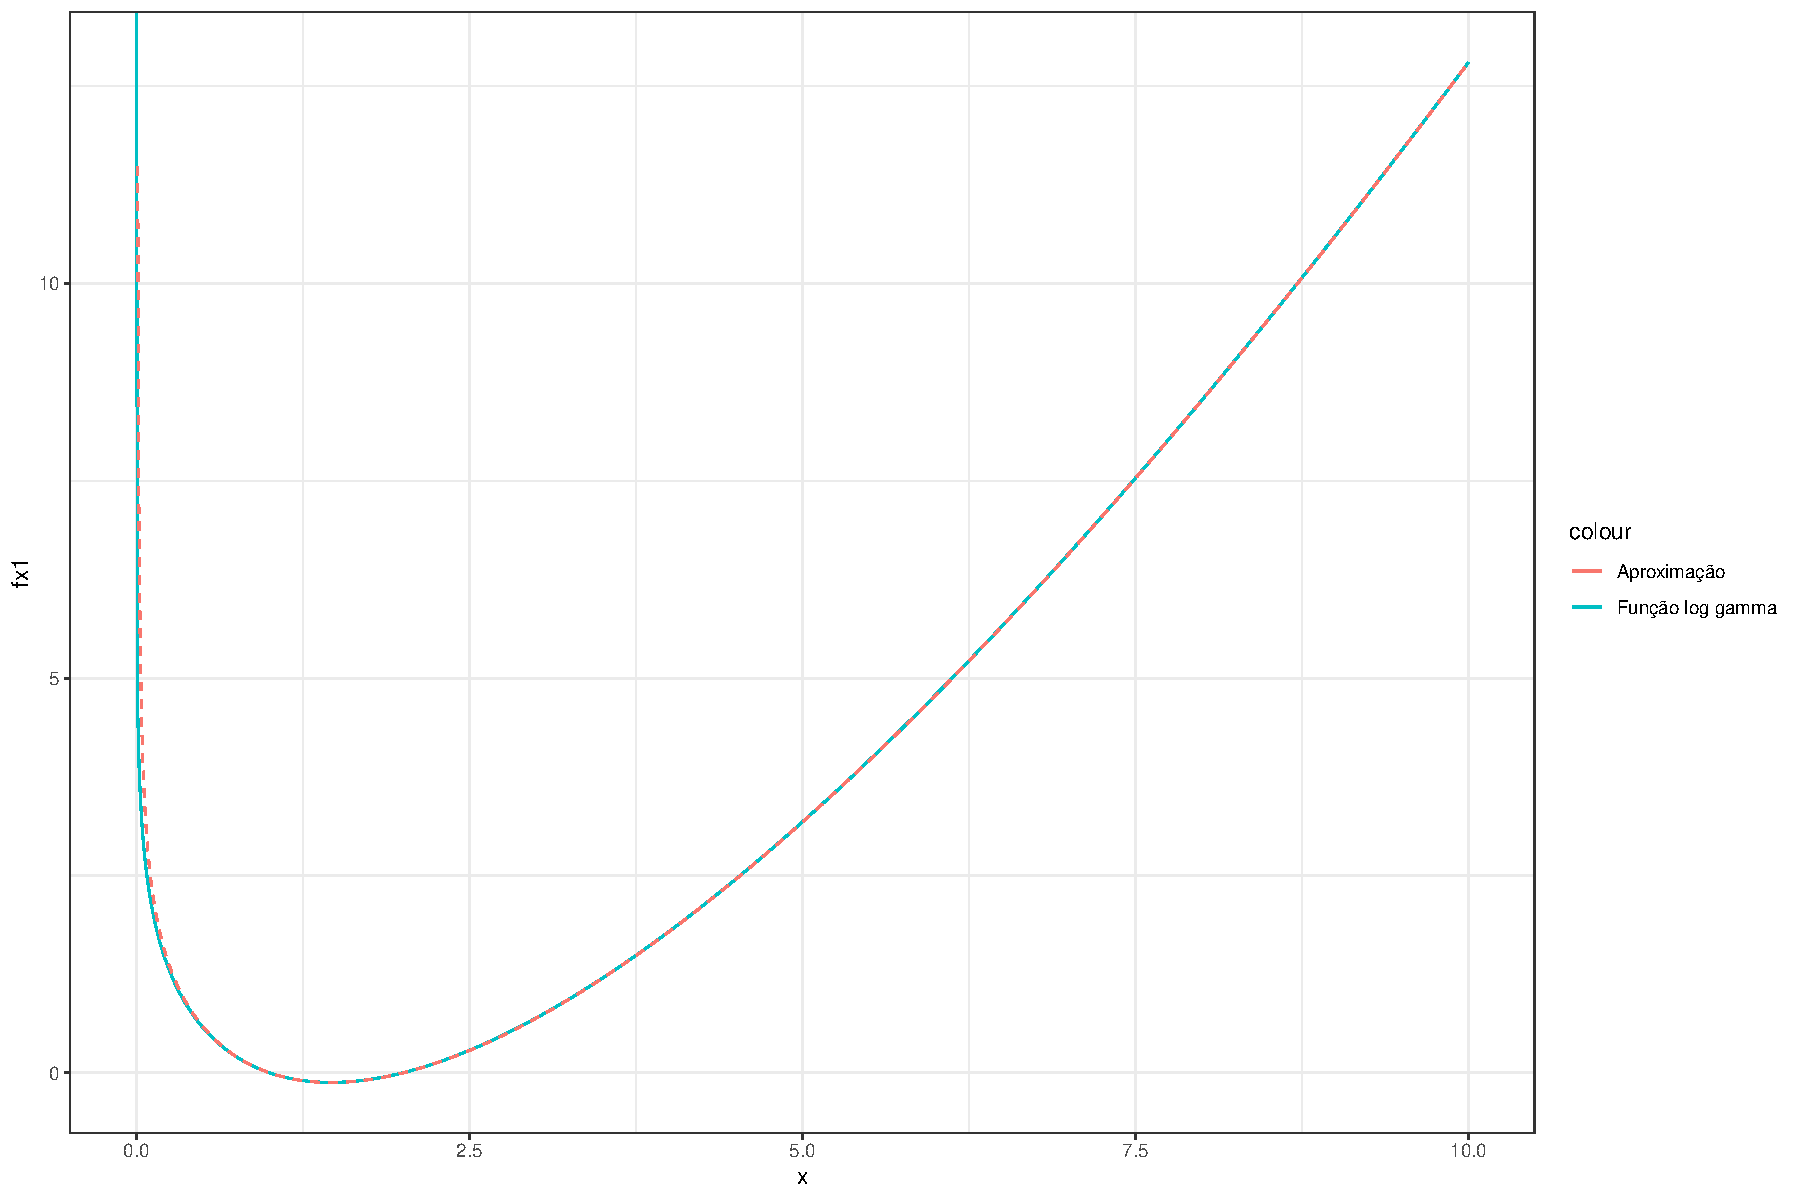
\includegraphics{caso_gamma_revisto_files/figure-latex/unnamed-chunk-1-1.pdf}

Em geral a aproximação parece boa, porém há certas ressalvas sobre o seu
uso, conforme discutirei mais à frente.

Calculemos então o valor esperado da última estatística suficiente
restante:

\[
\begin{aligned}
\mathbb{E}_{p^*}[\phi\ln(\phi)-\ln(\Gamma(\phi)]&\approx\mathbb{E}_{p^*}\left[\cancel{\phi\ln(\phi)}-\cancel{\phi\ln(\phi)}+\phi+\frac{1}{2}ln(\phi)-\frac{1}{12\phi}-\frac{11}{12}\right]\\
&=\frac{k^*_0+1}{2(n_0^*-k_0^*+n_0^*\ln\left(\frac{\tau_0}{n^*_0}\right)-\theta_0)}+\frac{1}{2}\left(\psi\left(\frac{k^*_0+1}{2}\right)-\ln\left(n_0^*-k_0^*+n_0^*\ln\left(\frac{\tau_0}{n^*_0}\right)-\theta_0\right)\right)\\
&-\frac{1}{12}\frac{2(n_0^*-k_0^*+n_0^*\ln\left(\frac{\tau_0}{n^*_0}\right)-\theta_0)}{k^*_0-1}-\frac{11}{12}.
\end{aligned}
\] \textbf{A aproximação acima é usada apenas quando
\(\frac{k_0^*+1}{2}\) é grande (maior que 3 já é o suficiente). Quando
\(\frac{k_0^*+1}{2}\) é pequeno, esse valor esperado é calculado usando
quadratura Gaussiana.}

As expressões aproximadas para
\(\mathbb{E}_{p^*}[-\phi(\psi(k^*_0\phi+1)-\ln(\phi\tau_0))]\) e
\(\mathbb{E}_{p^*}[\phi\ln(\phi)-\ln(\Gamma(\phi)]\) parecem bastente
úteis, porém elas tem um defeito muito grave: Elas não são válidas para
\(k_0^*\le1\). De fato, se \(k_0^*\le1\), \(\mathbb{E}_{p^*}[1/\phi]\)
não está definido, o que invalida as equações acima. Vale destacar que
\(\mathbb{E}_{p^*}[-\phi(\psi(k^*_0\phi+1)-\ln(\phi\tau_0))]\) e
\(\mathbb{E}_{p^*}[\phi\ln(\phi)-\ln(\Gamma(\phi)]\) \textbf{existem} e
são finitos, porém a aproximação da função \(\psi\) é ruim para valores
baixos de \(k_0^*\), especificamente, a aproximação de \(\psi\) é ruim
para valores pequenos de \(\phi\) e, quando \(k_0^*\) é pequeno, a
região onde a aproximação de \(\psi\) é ruim tem bastante massa de
probabilidade, de modo que a aproximação do valor esperado é ruim.

No caso em que trabalhamos no último relatório, \(\phi\) tinha
distribuição aproximada
\(\mathcal{G}\left(\frac{n_0+3}{2},n_0\ln\left(\frac{\tau_0}{n_0}\right)-\theta_0\right)\),
de modo que o parâmetro de forma era pelo menos \(1.5\), nesse caso, a
aproximação de \(\psi\) é sempre boa, mas, no caso atual, \(\phi\) tem
distribuição aproximada
\(\mathcal{G}\left(\frac{k^*_0+1}{2},n_0^*-k_0^*+n_0^*\ln\left(\frac{\tau_0}{n^*_0}\right)-\theta_0\right)\),
de modo que o parâmetro de forma é no mínimo \(0.5\), mas pode ser menor
que \(1.5\), de modo que a aproximação de \(\psi\) pode ser ruim.

De todo modo, a observação acima não é necessariamente um empecilho, uma
vez que podemos usar outros métodos para cálcular
\(\mathbb{E}_{p^*}[-\phi(\psi(k^*_0\phi+1)-\ln(\phi\tau_0))]\) e
\(\mathbb{E}_{p^*}[\phi\ln(\phi)-\ln(\Gamma(\phi)]\) sem aproximações.

Usando o novo sistema obtido, tentamos fazer o ajuste do modelo, porém
não conseguimos um ajuste funcional. Atualmente o problema com que
lidamos é que há casos onde o sistema
\(\mathbb{E}_{p^*}[H_{p^*}]=\mathbb{E}_{q}[H_{p^*}]\) tem solução.
Especificamente, há casos onde não existem parâmetros \(n^*_0\),
\(k^*_0\), \(\tau_0\) e \(\theta_0\) tais que a equação
\(\mathbb{E}_{p^*}[\phi\ln(\mu)]=\mathbb{E}_{q}[\phi\ln(\mu)]\) seja
verdadeira.

A partir de tudo que foi discutido, conseguimos escrever \(\theta_0\) e
\(\tau_0\) como funções de \(n^*_0\) e \(k^*_0\), de modo que as duas
primeiras equações do sistema sejam resolvidas (isto é, dado \(n^*_0\) e
\(k^*_0\), sabemos quem são os \(\theta_0\) e \(\tau_0\) que resolvem as
duas primeiras equações), assim precisamos apenas buscar \(n^*_0\) e
\(k^*_0\) que resolvam as duas últimas equações dado que \(\theta_0\) e
\(\tau_0\) são tais que as duas primeiras equações estão resolvidas.
Vamos analisar então \(\mathbb{E}_{p^*}[\phi\ln(\mu)]\) como funções de
\(n^*_0\) e \(k^*_0\):

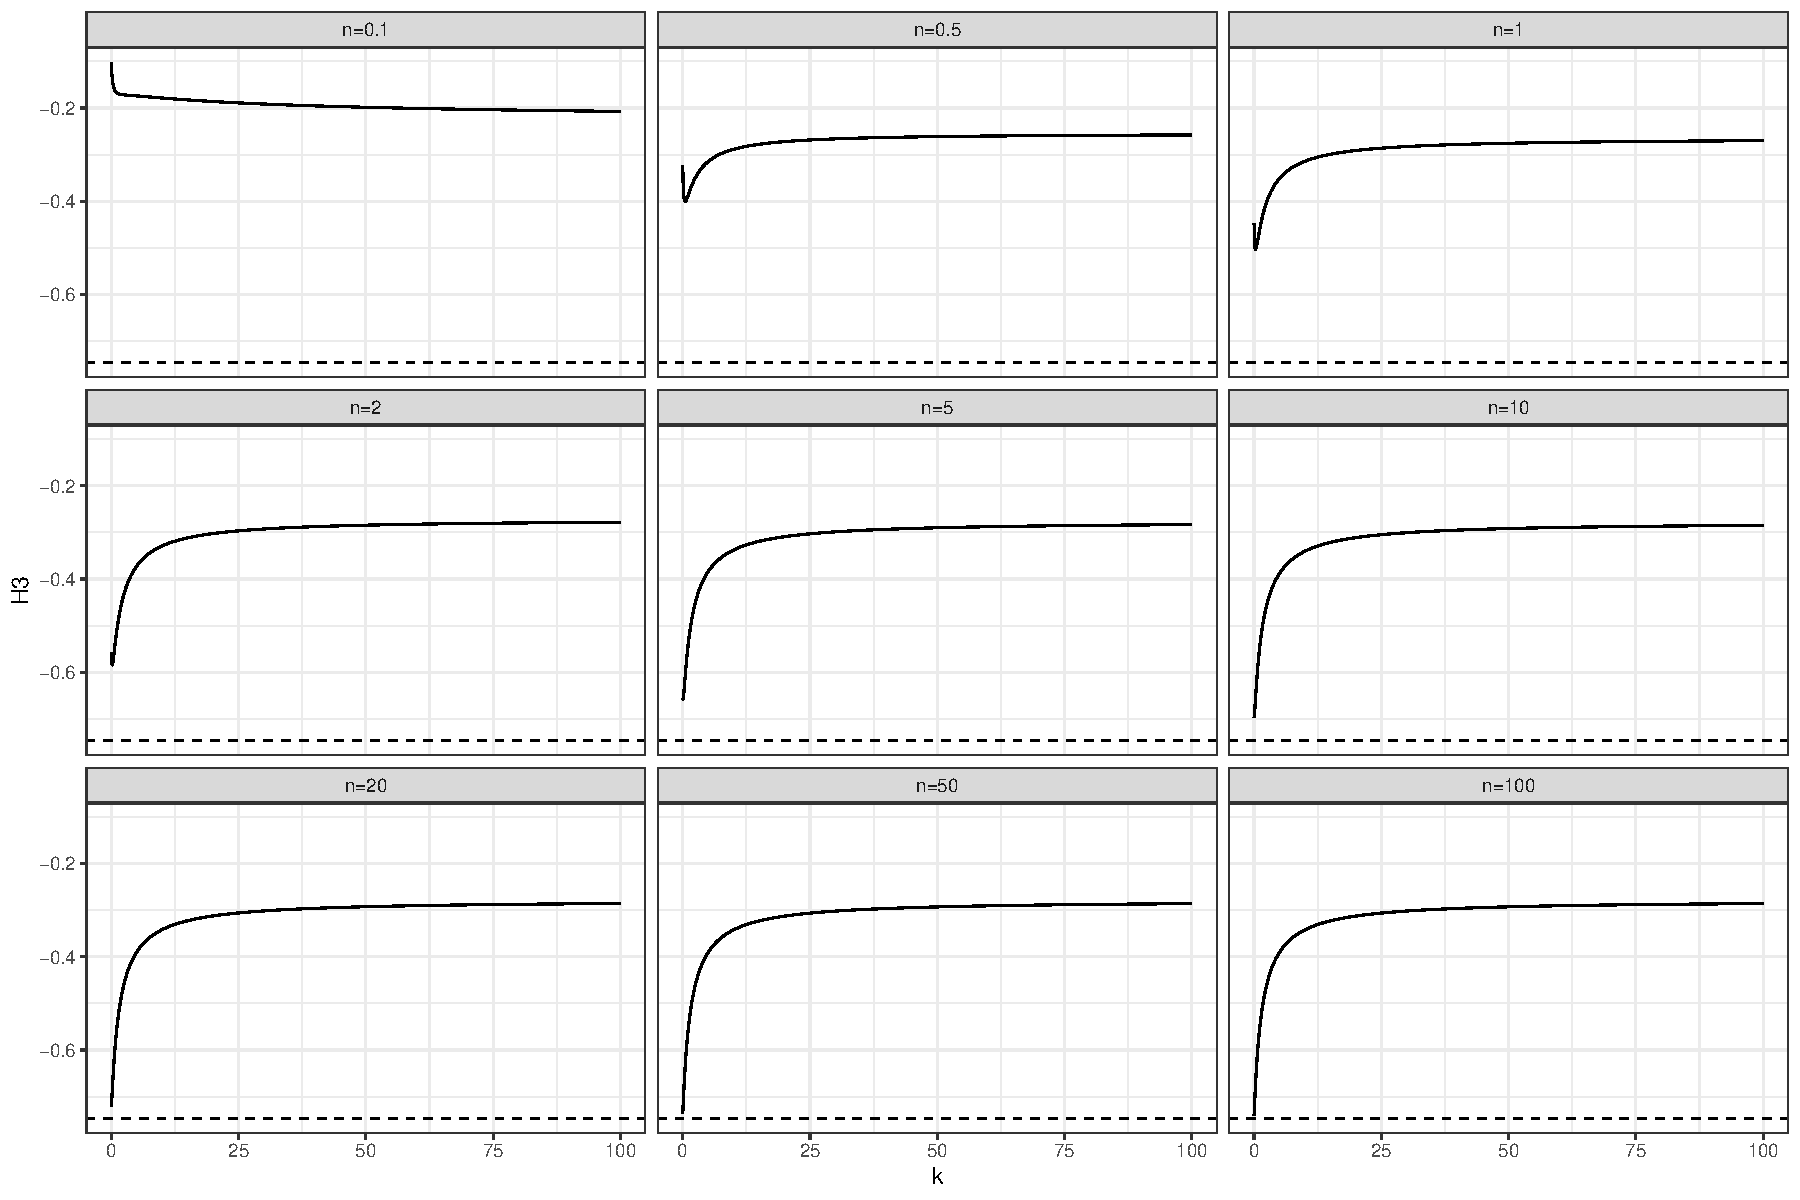
\includegraphics{caso_gamma_revisto_files/figure-latex/unnamed-chunk-3-1.pdf}

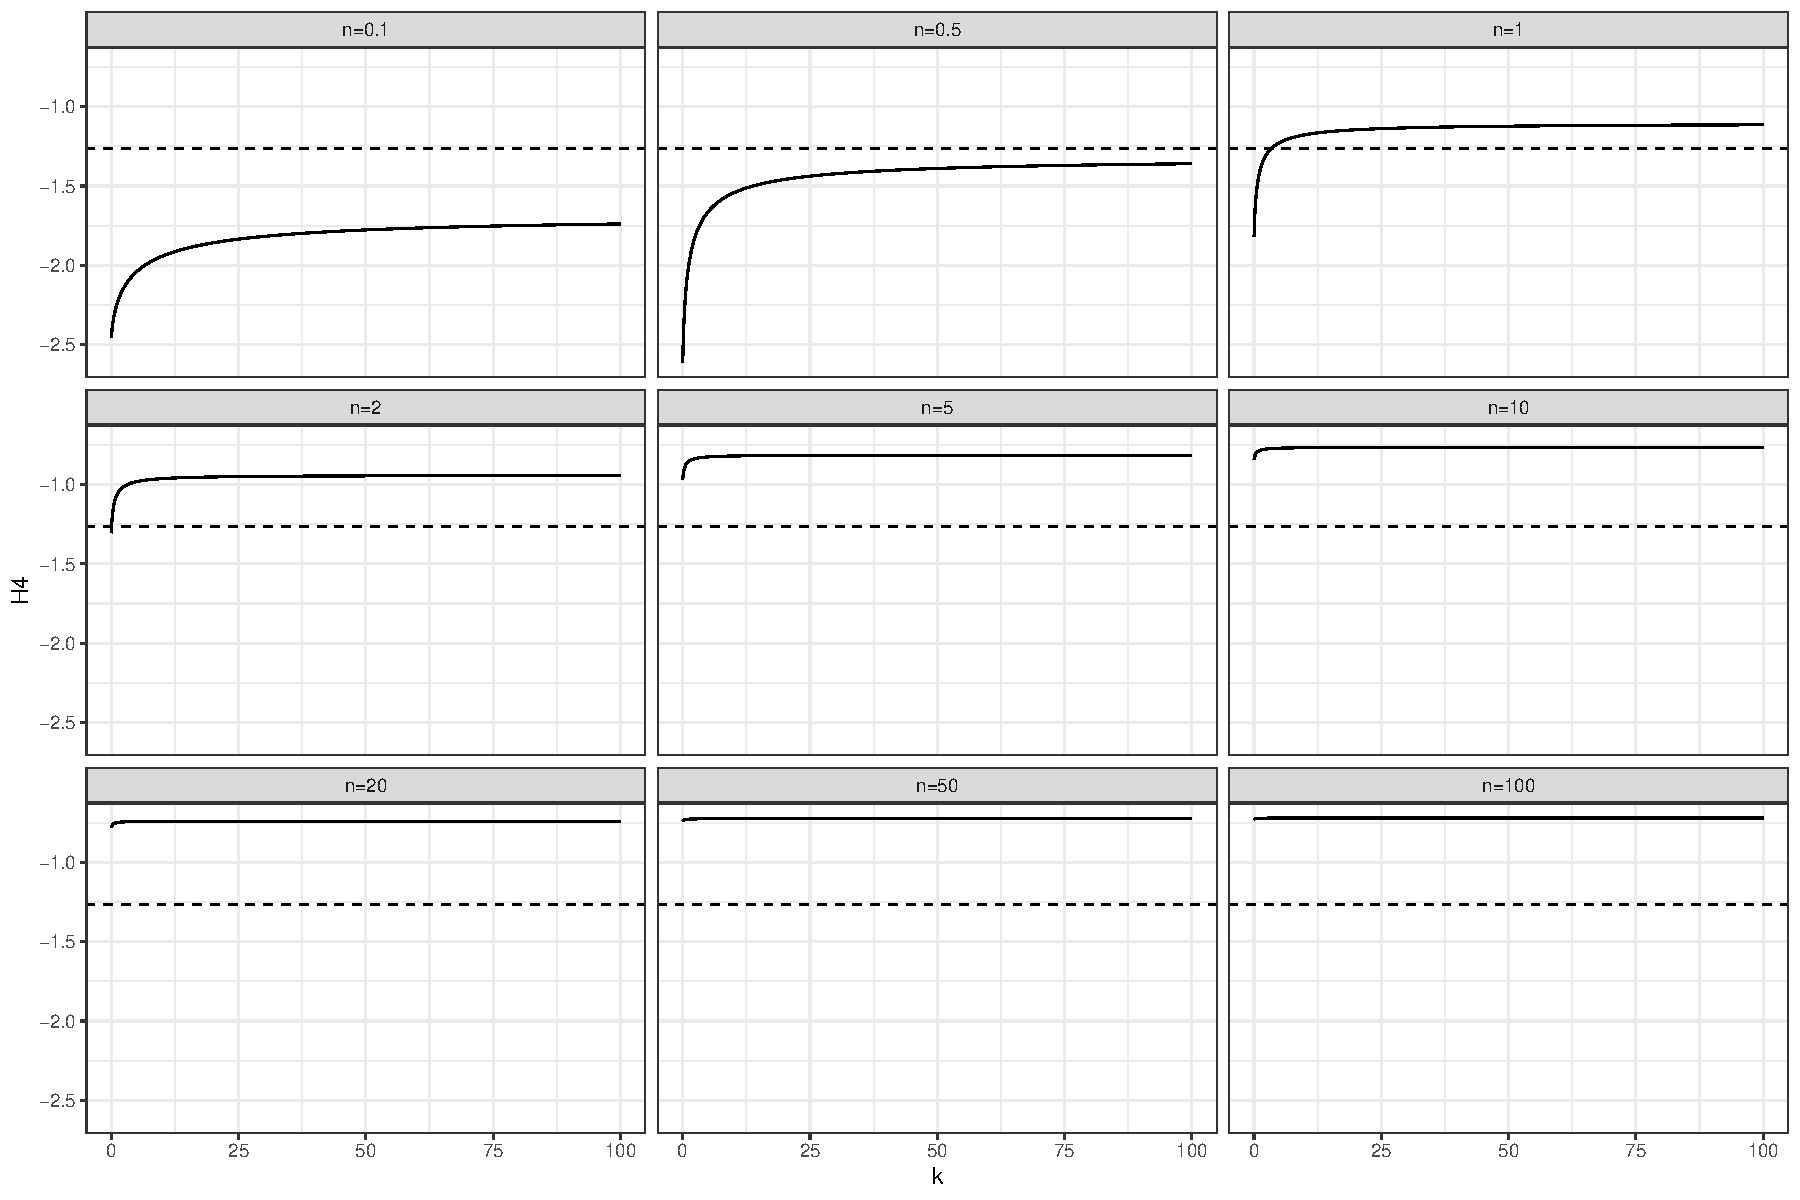
\includegraphics{caso_gamma_revisto_files/figure-latex/unnamed-chunk-4-1.pdf}

Temos, no final das contas, que \(\mathbb{E}_{p^*}[\phi\ln(\mu)]<0\),
para qualquer escolha de \(n^*_0\) ou \(k^*_0\), por outro lado, temos
que:

\[
\mathbb{E}_{q}[\phi\ln(\mu)]=-(f_2+q_{12})\exp\left\{f_1+\frac{q_1}{2}\right\},
\]

onde \(f_2\) é a média de \(\ln(\mu)\) na distribuição \(q\) (Normal
bivariada), \(q_{12}\) é a covariância de \(\ln(\phi)\) e \(\ln(\mu)\),
\(f_1\) é a média de \(\ln(\phi)\) e \(q_1\) é a variância de
\(\ln(\phi)\).

Veja que \(\mathbb{E}_{q}[\phi\ln(\mu)]\) pode ser positivo, basta que
\((f_2+q_{12})>0\), o que não pode ser evitado facilmente, de fato,
mesmo inicializando o processo em um ponto onde esta condição é válida,
pode acontecer de que esta condição seja violada eventualmente. Nesse
casos, o sistema \(\mathbb{E}_{p^*}[H_{p^*}]=\mathbb{E}_{q}[H_{p^*}]\)
\textbf{não} tem solução, pois sempre podemos diminuir a divergência
entre \(p\) e \(q\) tomando \(k^*_0\) cada vez maior. Na prática, o que
acontece ao longo do processo de resolução numérica do sistema é que o
algoritmo de Newton-Raphson diverge, com \(k^*_0\) indo para infinito.

No momento estou tentando encontrar alguma solução para o problema
acima.

\end{document}
